\documentclass[a4paper, 12pt]{article}

\usepackage{dblfnote}
\usepackage[perpage]{footmisc}
\usepackage{indentfirst}
\usepackage{framed}
\usepackage{tikz}
\usepackage{listings}[language=Python]
\usepackage{float}
\usepackage{subcaption}
\usepackage[square,numbers]{natbib}
%\usepackage{multicol}

\usepackage{setspace}
%\usepackage[skip=2mm, indent=17pt]{parskip}
\onehalfspacing
%\doublespacing


% Custom colors
\usepackage{color}

%\setcounter{secnumdepth}{0}

\usepackage[top=3cm, bottom=3cm, left = 2cm, right = 2cm]{geometry} 
\geometry{a4paper} 
\usepackage{url}
\usepackage{graphicx} 
\usepackage{amsmath,amssymb}  
\usepackage[hidelinks]{hyperref}
\usepackage[labelformat=empty]{caption}
\usepackage{xepersian}
\settextfont{XB Yas}
\usepackage[utf8]{inputenc}

%\usepackage{xepersian}

\DeclareFixedFont{\ttb}{T1}{txtt}{bx}{n}{12} % for bold
\DeclareFixedFont{\ttm}{T1}{txtt}{m}{n}{12}  % for normal

\definecolor{deepblue}{rgb}{0,0,0.5}
\definecolor{deepred}{rgb}{0.6,0,0}
\definecolor{deepgreen}{rgb}{0,0.5,0}

\newcommand\pythonstyle{\lstset{
		language=Python,
		basicstyle=\ttm,
		morekeywords={self},              % Add keywords here
		keywordstyle=\ttb\color{deepblue},
		emph={MyClass,__init__},          % Custom highlighting
		emphstyle=\ttb\color{deepred},    % Custom highlighting style
		stringstyle=\color{deepgreen},
		frame=single,                         % Any extra options here
		showstringspaces=false
}}


% Python environment
\lstnewenvironment{python}[1][]
{
	\pythonstyle
	\lstset{#1}
}
{}

% Python for external files
\newcommand\pythonexternal[2][]{{
		\pythonstyle
		\lstinputlisting[#1]{#2}}}

% Python for inline
\newcommand\pythoninline[1]{{\pythonstyle\lstinline!#1!}}




\begin{document}	
	\noindent
	\begin{minipage}[c]{5cm}
		\baselineskip=.7cm
		\begin{flushright}
			درس : مباحث ویژه در داده‌کاوی
			\\
			دانشجو :
			امیرمحمد خرازی
			\\
			شماره دانشجویی :
			40152521002 
			\\
			استاد درس :  
			\href{mrezghi.ir}{دکتر منصور رزقی آهق}
		\end{flushright}
	\end{minipage}
	\hfill
	\begin{minipage}[c]{3cm}
		\begin{center}
			\href{modares.ac.ir}{
				
\includegraphics[width=2cm]{logo.png}}
		\end{center}	
	\end{minipage}
	\\[1mm]
	\hrule depth .5mm \relax
	\begin{flushright}
		تمرین سوم
		\hfill
		دانشکده علوم ریاضی ، گروه علوم کامپیوتر، گرایش داده‌کاوی
		\\
		\vspace{5mm}
		گیت‌هاب درس (
		\href{https://github.com/A-M-Kharazi/Special-Topics-in-DataMining-TMU.git}{لینک}
		)
		\hfill
		گیت‌هاب این تمرین (
		\href{}{لینک}
		)
	\end{flushright}
	
	\hrule depth .5mm\relax
	
	%\tableofcontents
	%\newpage
	
	\section*{اطلاعات اضافی}
	گزارش کامل‌تر داخل کد‌‌ها آورده شده است . بطور کلی هدف تقریب یک عکس سیاه و سفید با استفاده از SVD و بررسی وضعیت بردار‌های U در این تقریب هستیم. عکس مورد استفاده عکس فیلمبردار یا cameraman است که از sklearn قابل دسترسی است. ۸ نمونه از تقریب های آن را در اینجا مشاهده می‌کنید :
	\begin{center}
		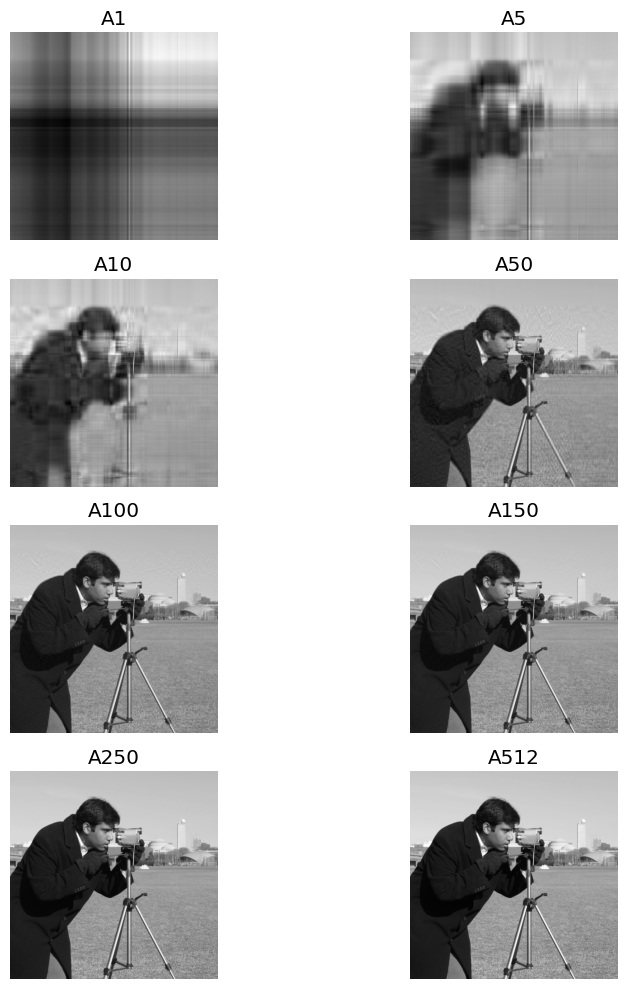
\includegraphics[scale=0.5]{fig1.png}
	\end{center}
	همچنین وضعیت U ها را می‌توانید در این تصویر مشاهده کنید :
	\begin{center}
		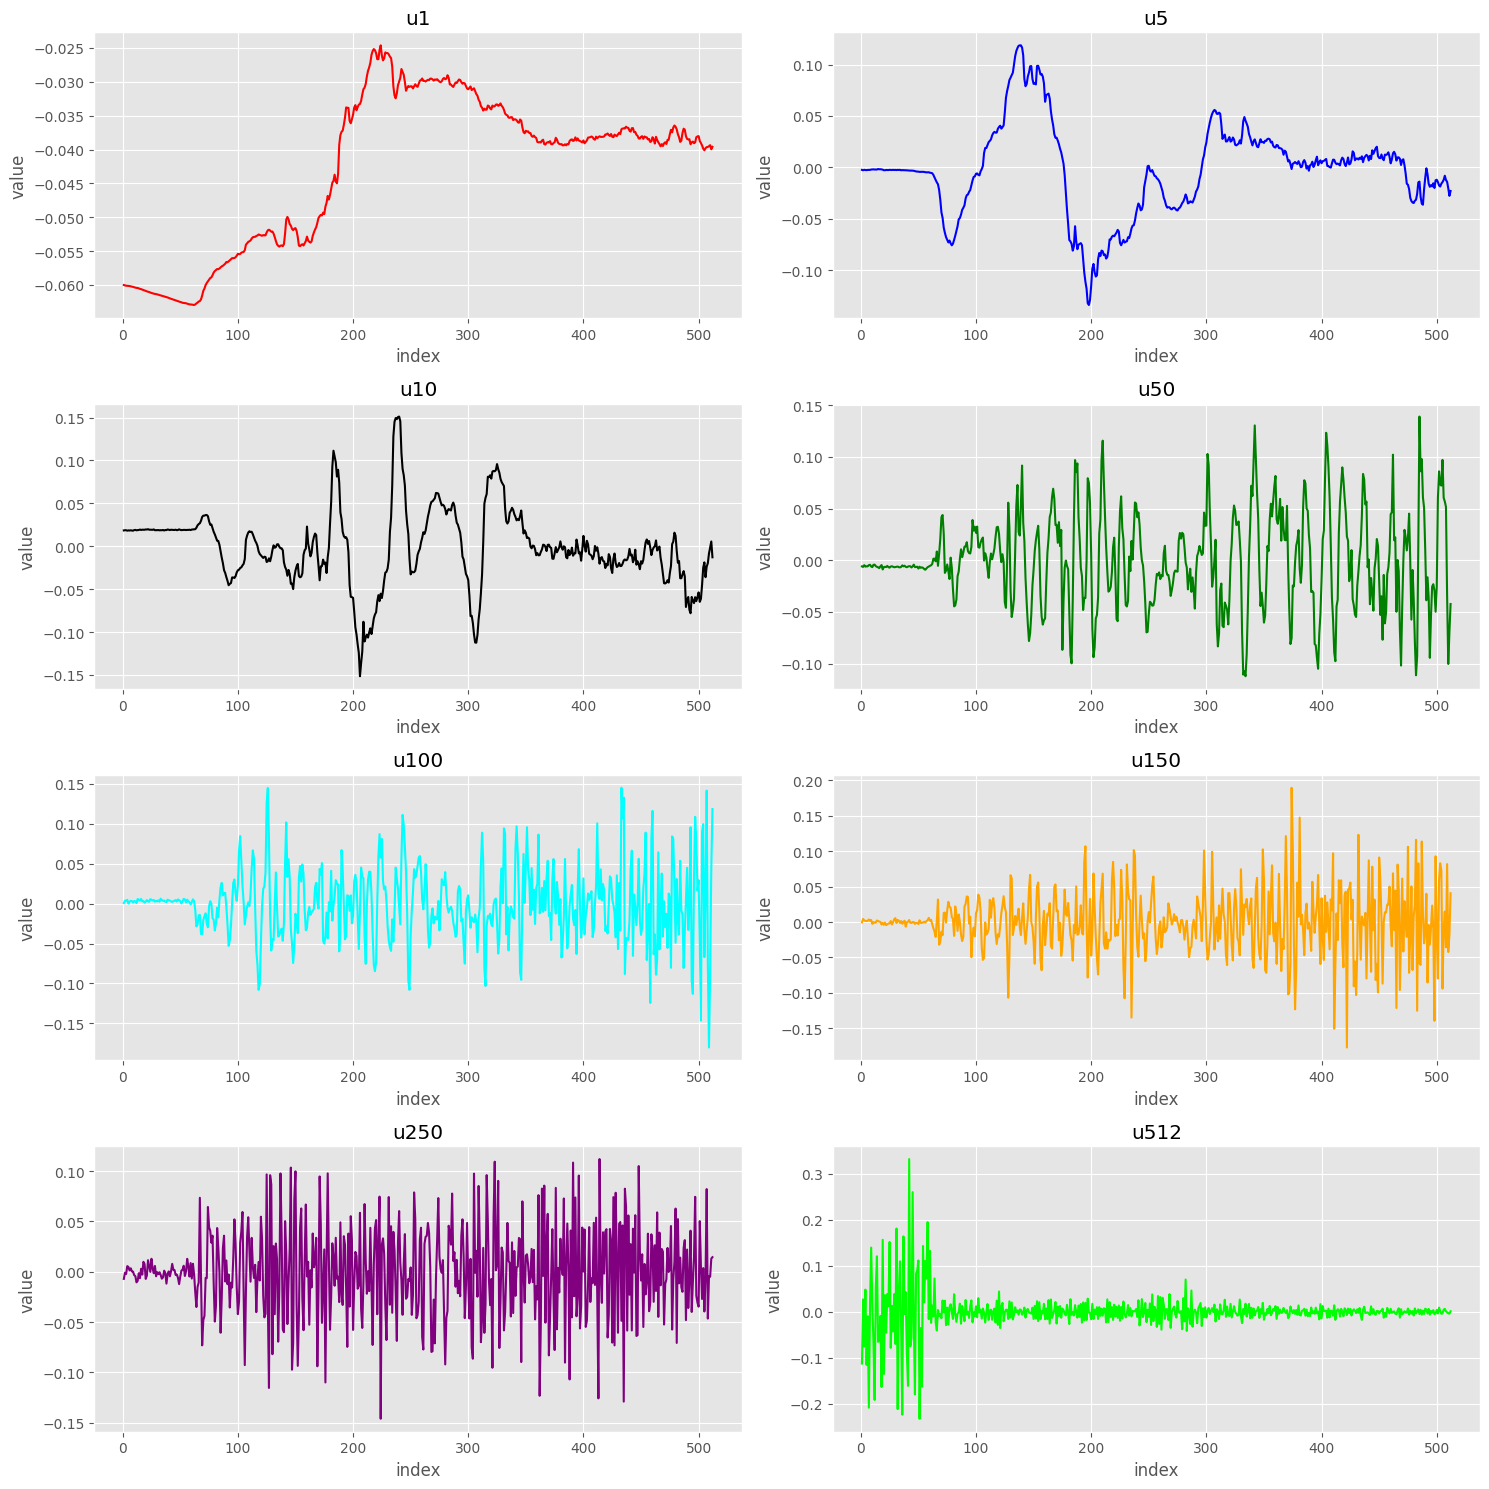
\includegraphics[scale=0.4]{fig2.png}
	\end{center}
	
	از طرفی تصویر بعد از اضافه کردن نویز و تقریب‌های آن بصورت زیر خواهد بود :
	\begin{center}
		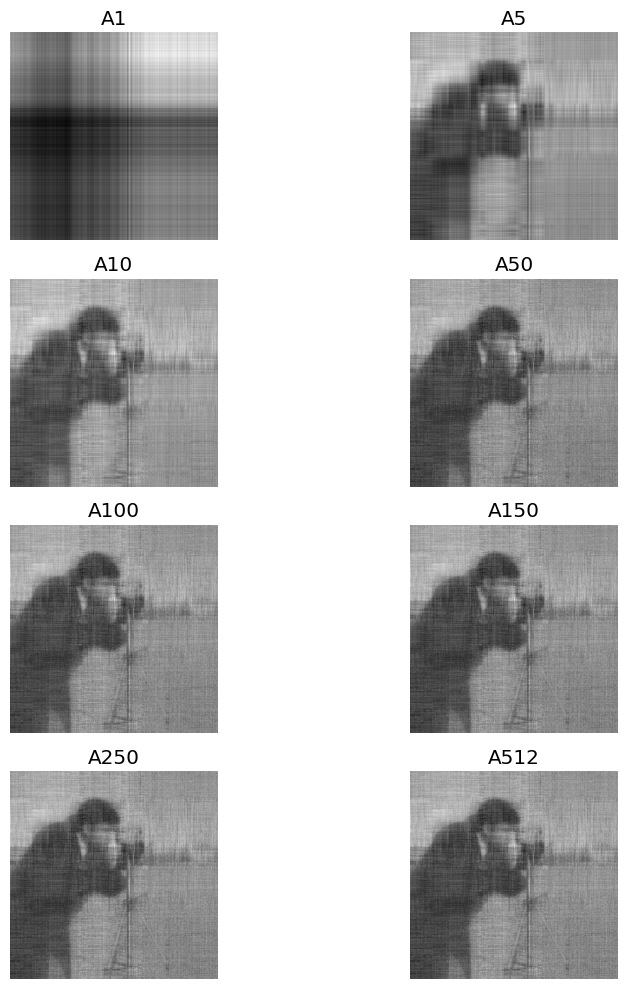
\includegraphics[scale=0.5]{fig3.png}
	\end{center}
و وضعیت U های آن بشکل زیر است :
\begin{center}
	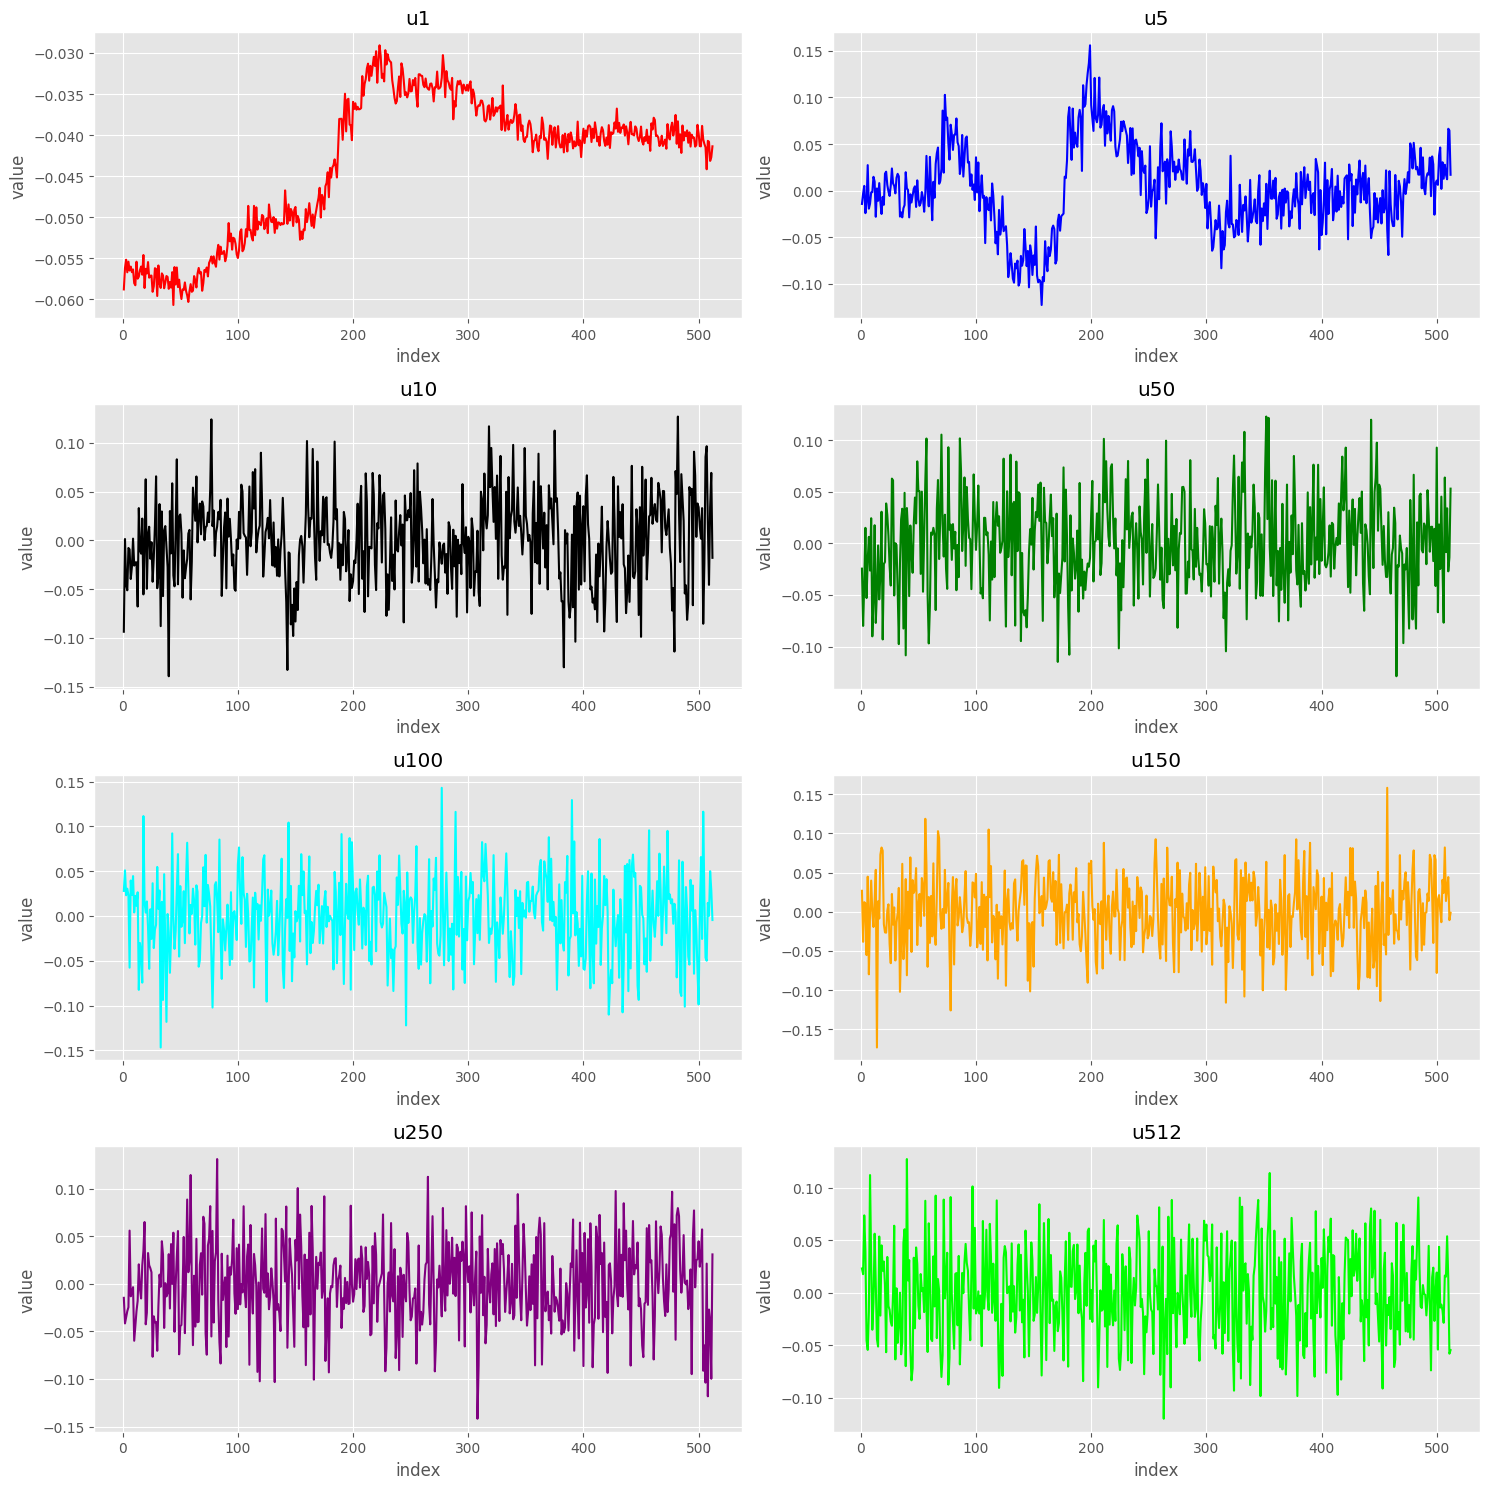
\includegraphics[scale=0.4]{fig4.png}
\end{center}
مشاهده می‌شود که بسیاری از نویز ها در U های آخر نشسته است . البته در U های اولیه هم نویز دیده می‌شود ولی در آخر بیشتر است. 

همچنین می‌توان نمودار مربوط به مقادیر تکین را رسم کرد که اندازه آن‌ها در مقایسه با تصویر اصلی کاهش یافته است.
\begin{center}
	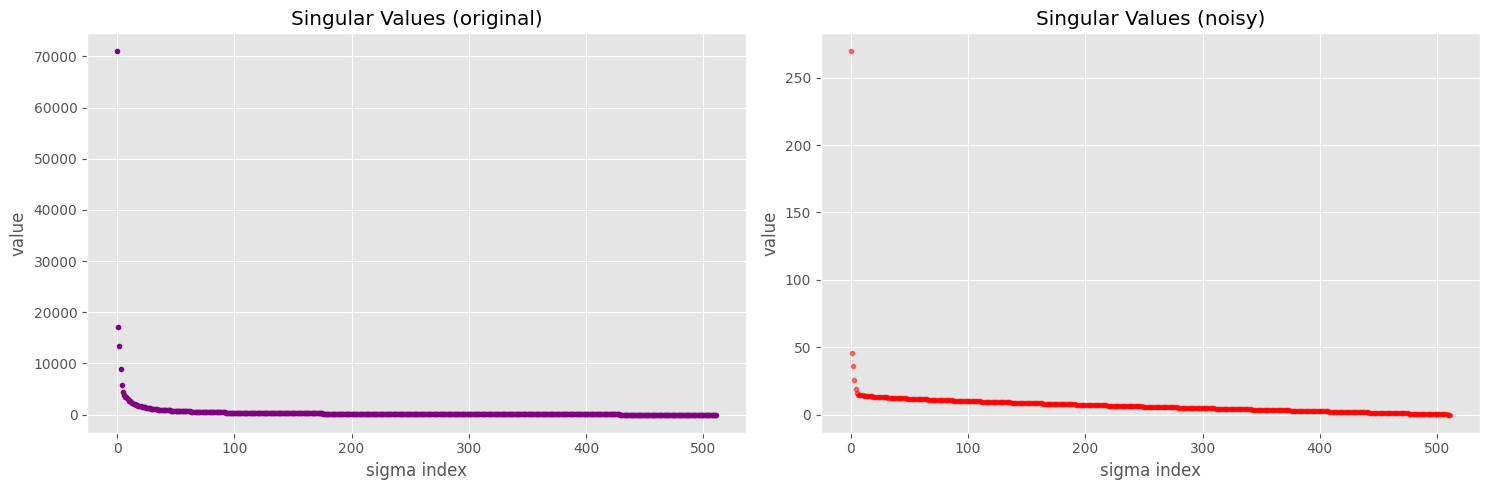
\includegraphics[scale=0.4]{fig5.png}
\end{center}

جزئیات کد در فایل مربوطه قابل بررسی است.

\textbf{خروجی ها در گیت‌هاب پاک شده است (بدلیل حجم زیاد آن‌ها). اگر از گیت‌هاب آن را باز می‌کنید باید از کد‌ها اجرا بگیرید که بعضی بخش های آن زمان بر است.}
	
	
\end{document}


